%% BioMed_Central_Tex_Template_v1.06
%%                                      %
%  ms00_bmc_article.tex            ver: 1.06 %
%                                       %

%%IMPORTANT: do not delete the first line of this template
%%It must be present to enable the BMC Submission system to
%%recognise this template!!

%%%%%%%%%%%%%%%%%%%%%%%%%%%%%%%%%%%%%%%%%
%%                                     %%
%%  LaTeX template for BioMed Central  %%
%%     journal article submissions     %%
%%                                     %%
%%          <8 June 2012>              %%
%%                                     %%
%%                                     %%
%%%%%%%%%%%%%%%%%%%%%%%%%%%%%%%%%%%%%%%%%

%%%%%%%%%%%%%%%%%%%%%%%%%%%%%%%%%%%%%%%%%%%%%%%%%%%%%%%%%%%%%%%%%%%%%
%%                                                                 %%
%% For instructions on how to fill out this Tex template           %%
%% document please refer to Readme.html and the instructions for   %%
%% authors page on the biomed central website                      %%
%% https://www.biomedcentral.com/getpublished                      %%
%%                                                                 %%
%% Please do not use \input{...} to include other tex files.       %%
%% Submit your LaTeX manuscript as one .tex document.              %%
%%                                                                 %%
%% All additional figures and files should be attached             %%
%% separately and not embedded in the \TeX\ document itself.       %%
%%                                                                 %%
%% BioMed Central currently use the MikTex distribution of         %%
%% TeX for Windows) of TeX and LaTeX.  This is available from      %%
%% https://miktex.org/                                             %%
%%                                                                 %%
%%%%%%%%%%%%%%%%%%%%%%%%%%%%%%%%%%%%%%%%%%%%%%%%%%%%%%%%%%%%%%%%%%%%%

%%% additional documentclass options:
%  [doublespacing]
%  [linenumbers]   - put the line numbers on margins

%%% loading packages, author definitions

%\documentclass[twocolumn]{bmcart}% uncomment this for twocolumn layout and comment line below
\documentclass[doublespacing,linenumbers]{bmcart}

% Set relative path to all figures
\newcommand*{\floatRelativePath}{../out/gwas417/pval_5e-08/r2_0.1/kb_1000/window_1000000/75_25}%

%%% Load packages
\usepackage{amsthm,amsmath}
%\RequirePackage[numbers]{natbib}
%\RequirePackage[authoryear]{natbib}% uncomment this for author-year bibliography
\RequirePackage{hyperref}
\usepackage[utf8]{inputenc} %unicode support
%\usepackage[applemac]{inputenc} %applemac support if unicode package fails
%\usepackage[latin1]{inputenc} %UNIX support if unicode package fails

\usepackage{csvsimple}

%%%%%%%%%%%%%%%%%%%%%%%%%%%%%%%%%%%%%%%%%%%%%%%%%
%%                                             %%
%%  If you wish to display your graphics for   %%
%%  your own use using includegraphic or       %%
%%  includegraphics, then comment out the      %%
%%  following two lines of code.               %%
%%  NB: These line *must* be included when     %%
%%  submitting to BMC.                         %%
%%  All figure files must be submitted as      %%
%%  separate graphics through the BMC          %%
%%  submission process, not included in the    %%
%%  submitted article.                         %%
%%                                             %%
%%%%%%%%%%%%%%%%%%%%%%%%%%%%%%%%%%%%%%%%%%%%%%%%%

\def\includegraphic{}
\def\includegraphics{}

%%% Put your definitions there:
\startlocaldefs
\endlocaldefs

%%% Begin ...
\begin{document}

%%% Start of article front matter
    \begin{frontmatter}

%        \begin{fmbox}
            \dochead{Research}

%%%%%%%%%%%%%%%%%%%%%%%%%%%%%%%%%%%%%%%%%%%%%%
%%                                          %%
%% Enter the title of your article here     %%
%%                                          %%
%%%%%%%%%%%%%%%%%%%%%%%%%%%%%%%%%%%%%%%%%%%%%%

            \title{Pleiotropy of expression quantitative trait loci increases with the number of regulated genes, active cell types and tissues and bound transcription factors}

%%%%%%%%%%%%%%%%%%%%%%%%%%%%%%%%%%%%%%%%%%%%%%
%%                                          %%
%% Enter the authors here                   %%
%%                                          %%
%% Specify information, if available,       %%
%% in the form:                             %%
%%   <key>={<id1>,<id2>}                    %%
%%   <key>=                                 %%
%% Comment or delete the keys which are     %%
%% not used. Repeat \author command as much %%
%% as required.                             %%
%%                                          %%
%%%%%%%%%%%%%%%%%%%%%%%%%%%%%%%%%%%%%%%%%%%%%%

            \author[
                addressref={aff1},                   % id's of addresses, e.g. {aff1,aff2}
                corref={aff1},                       % id of corresponding address, if any
% noteref={n1},                        % id's of article notes, if any
                email={aitor.gonzalez@univ-amu.fr}   % email address
            ]{\inits{A.G.}\fnm{Aitor} \snm{González}}
%\author[
%  addressref={aff1,aff2},
%  email={john.RS.Smith@cambridge.co.uk}
%]{\inits{J.R.S.}\fnm{John R.S.} \snm{Smith}}

%%%%%%%%%%%%%%%%%%%%%%%%%%%%%%%%%%%%%%%%%%%%%%
%%                                          %%
%% Enter the authors' addresses here        %%
%%                                          %%
%% Repeat \address commands as much as      %%
%% required.                                %%
%%                                          %%
%%%%%%%%%%%%%%%%%%%%%%%%%%%%%%%%%%%%%%%%%%%%%%

            \address[id=aff1]{%                           % unique id
%  \orgdiv{Department of Science},             % department, if any
                \orgname{Aix Marseille Univ, INSERM, TAGC},          % university, etc
                \city{Marseille},                              % city
                \cny{France}                                    % country
            }
%\address[id=aff2]{%
%  \orgdiv{Institute of Biology},
%  \orgname{National University of Sciences},
%  %\street{},
%  %\postcode{}
%  \city{Kiel},
%  \cny{Germany}
%}

%%%%%%%%%%%%%%%%%%%%%%%%%%%%%%%%%%%%%%%%%%%%%%
%%                                          %%
%% Enter short notes here                   %%
%%                                          %%
%% Short notes will be after addresses      %%
%% on first page.                           %%
%%                                          %%
%%%%%%%%%%%%%%%%%%%%%%%%%%%%%%%%%%%%%%%%%%%%%%

%\begin{artnotes}
%%\note{Sample of title note}     % note to the article
%\note[id=n1]{Equal contributor} % note, connected to author
%\end{artnotes}

%        \end{fmbox}% comment this for two column layout

%%%%%%%%%%%%%%%%%%%%%%%%%%%%%%%%%%%%%%%%%%%%%%%
%%                                           %%
%% The Abstract begins here                  %%
%%                                           %%
%% Please refer to the Instructions for      %%
%% authors on https://www.biomedcentral.com/ %%
%% and include the section headings          %%
%% accordingly for your article type.        %%
%%                                           %%
%%%%%%%%%%%%%%%%%%%%%%%%%%%%%%%%%%%%%%%%%%%%%%%

%        \begin{abstractbox}

            \begin{abstract} % abstract

                \parttitle{Background} %if any
                %
                Pleiotropic genetic variants affecting several traits are relatively common in the genome as shown by the increasing number of genome-wide association studies (GWAS).
%
                Complex disease variants are often located in non-coding regions and are likely gene regulatory variants.
%
                In this work, I investigate the link between frequent expression quantitative trait loci and pleiotropy.

                \parttitle{Results} %if any
% Verify numbers
                First I have computed the colocalization probability of 417 GWAS and 127 eQTL studies and I have observed 10,334 GWAS/eQTL pairs with at least one colocalized variants with a probability above 0.8.
%SELECT count(DISTINCT concat(`gwas_id`, `eqtl_id`)) FROM `gwas2eqtl_modelgwas2eqtl` where `PP_H4_abf`>=0.8; 10334
%Pourcentage of GWAS
%
                I have categorized the GWAS traits into 96 traits and categories to define pleiotropic as belonging at least to two of these categories.
%
                Pleiotropic variants are associated to more eQTL genes (eGenes) and more eQTL tissues (etissues) but egenes do also correlate with more traits.
%
                These observations could be partially explained, because pleitropic variants are enriched in splicing and missense variants and bind more transcription factors.
%
                These variants with the GWAS traits, egenes and etissues can be explored in a public website.

                \parttitle{Conclusions} %if any
                In conclusion, our work suggest that pleiotropy of gene regulatory variants arise from an increase of bound transcription factors, target egenes and etissues and severity of molecular effect consequences.
                %
            \end{abstract}

%%%%%%%%%%%%%%%%%%%%%%%%%%%%%%%%%%%%%%%%%%%%%%
%%                                          %%
%% The keywords begin here                  %%
%%                                          %%
%% Put each keyword in separate \kwd{}.     %%
%%                                          %%
%%%%%%%%%%%%%%%%%%%%%%%%%%%%%%%%%%%%%%%%%%%%%%

            \begin{keyword}
                \kwd{genetic variants}
                \kwd{expression quantitative trait loci}
                \kwd{complex diseases}
                \kwd{pleiotropy}
            \end{keyword}

% MSC classifications codes, if any
%\begin{keyword}[class=AMS]
%\kwd[Primary ]{}
%\kwd{}
%\kwd[; secondary ]{}
%\end{keyword}

%        \end{abstractbox}
%
%\end{fmbox}% uncomment this for two column layout

    \end{frontmatter}

%%%%%%%%%%%%%%%%%%%%%%%%%%%%%%%%%%%%%%%%%%%%%%%%
%%                                            %%
%% The Main Body begins here                  %%
%%                                            %%
%% Please refer to the instructions for       %%
%% authors on:                                %%
%% https://www.biomedcentral.com/getpublished %%
%% and include the section headings           %%
%% accordingly for your article type.         %%
%%                                            %%
%% See the Results and Discussion section     %%
%% for details on how to create sub-sections  %%
%%                                            %%
%% use \cite{...} to cite references          %%
%%  \cite{koon} and                           %%
%%  \cite{oreg,khar,zvai,xjon,schn,pond}      %%
%%                                            %%
%%%%%%%%%%%%%%%%%%%%%%%%%%%%%%%%%%%%%%%%%%%%%%%%

%%%%%%%%%%%%%%%%%%%%%%%%% start of article main body
% <put your article body there>

%%%%%%%%%%%%%%%%
%% Background %%

    \section*{Introduction}\label{sec:introduction}

% GWAS in general
Genome-wide association studies (GWAS) have allowed the association of frequent genetic variants with common traits.
%
The number of GWAS has rapidly increased since the first GWAS around 15 years ago and has resulted in comprehensive databases such as the NHGRI-EBI GWAS Catalog \cite{2007burton.barret,2018.Parkinson.Buniello}.
%
For instance, in 2019, NHGRI-EBI GWAS Catalog contained 5687 GWAS comprising 71,673 variant-trait associations from 3,567 publications \cite{2018.Parkinson.Buniello}.

% Shortcomings of GWAS
However, the interpretation of the GWAS variants is complex because of three reasons \cite{2020.Trynka.CanoGamez}.
%
First, the causal variant is hidden in regions with high linkage disequilibrium (LD).
%
Second, GWAS do not inform about the genes, cell types, and tissues involved in the phenotypes.
%
Third, GWAS variants often affect non-coding regions, where the molecular cause is more difficult to define.

% Interest in studying GWAS
Expression QTLs (eQTLs) are variants that change the expression of a given gene in a cell type or tissue.
%
eQTLs share some of the same shortcomings as GWAS variants such as the inability to identify the causal variant in regions of high LD.
%
Moreover, the distribution of eQTLs and GWAS variants in the genome are different because of negative selection \cite{2022.Pritchard.Mostafavi}.
%
Nevertheless, eQTLs are still important data sets to interpret GWAS variants, because they provide gene regulatory information about the eQTL genes and cell types and tissues \cite{2021.Li.Mu}.
%
%In addition, colocalization analysis can help prioritize causal variants.

Many GWAS have allowed observing that many genetic variants are involved in different traits \cite{2019.Posthuma.Watanabe}.
%
In that work, the analyzed loci covered 60\% of the genome, and 90\% of these loci contained associations across different traits \cite{2019.Posthuma.Watanabe}.
%
They also found that pleiotropic genes and variants were less tissue-specific in terms of gene expression and eQTLs \cite{2019.Posthuma.Watanabe}.
%
However, the question of tissue specificity of eQTLs has been analyzed in different works with conflicting conclusions \cite{2021.Li.Mu,2018.Vijayanand.Schmiedel,2017gtex.nature}.
%
In addition, the mechanism of pleiotropy is not well understood yet.

In this work, I have taken advantage of two large eQTL and GWAS data sets from the EBI eQTL Catalogue and the IEU OpenGWAS, respectively,
to develop a global colocalization analysis based on 127 eQTL studies and 418 GWAS across many cell types, tissues, and phenotypes.
%
I have used these eQTL/GWAS variants to investigate mechanisms of pleiotropic gene regulatory variants.
%
These eQTL/GWAS variants might be a useful resource for the annotation and prioritization of frequent variants.
%
Therefore, I have developed an easy-to-use web application to expose these colocalization data.

    \section*{Results}\label{s:results}

%%%%%%%%%%%%%%%%%%%%%%%%%%%%%%%%%%%%%%%%%%%%%%%%%%%%%%%%%%%%%%%%%%%%%%%%%%%%%%%%%%%%%%%%%%%%%%%%%%%%%%%%%%%%%%%%%%%%%%%%
%
\subsection*{Systematic colocalization of variants from genome-wide associations studies and expression quantitative trait loci}
%
%%%%%%%%%%%%%%%%%%%%%%%%%%%%%%%%%%%%%%%%%%%%%%%%%%%%%%%%%%%%%%%%%%%%%%%%%%%%%%%%%%%%%%%%%%%%%%%%%%%%%%%%%%%%%%%%%%%%%%%%

To annotate traits from genome-wide associations studies (GWAS) with genes and tissues,
I developed a pipeline that systematically colocalizes variants from GWAS and expression quantitative trait loci (eQTLs) (Section Methods).
%
% TODO Supplementary table 1 for newest pipeline
127 eQTL studies were downloaded from the EBI eQTL catalogue, which aims to provide uniformly processed eQTLs in many
tissues and cell types \citep{2021.Alasoo.Kerimov} (Supplementary table 1).

GWAS traits were selected from the IEU OpenGWAS database based on four criteria \citep{2018.Parkinson.Buniello}.
%
The first criterion was to exclude molecular traits such as proteome or methylome.
%	
The second criterion was to include only the European population, because most
samples from the EBI eQTL catalogue belong to the European population.
%
The third criterion was to keep only well-defined medical or physiological
conditions and exclude environmental traits such "employment status" or "self-reported" medical conditions.
%
The fourth criterion was to keep only GWAS with at least 10,000 subjects, 2,000 controls and 2,000 cases.
%
% TODO Supplementary table 2 for newest pipeline
These filters resulted in 418 GWAS traits (Supplementary table 2).
%
Among these studies, there were 8,580 clumped leading variants with a p-value below 5e-8 from 284 GWAS (Supplementary file).
% select count(distinct gwas_id) from tophits; 284
% select count(*) from (select DISTINCT chrom, pos, rsid, ea from tophits) as sel; 8,580
% tophits goes to OSF
% colocpleio goes to OSF

My pipeline uncovered eQTL colocalizations for 5,484 or 64$\%$ of the leading GWAS variants with 7,040 eQTL genes and 127 eQTL biosamples.
% select count(*) from (select distinct tophits.rsid from tophits inner join coloc on coloc.rsid=tophits.rsid where coloc.pp_h4_abf>=0.75) as sel; 5484
% select count(*) from (select distinct eqtl_gene_id from coloc where pp_h4_abf>=0.75) as sel;  7040
% select count(*) from (select distinct eqtl_id from coloc where pp_h4_abf>=0.75) as sel;  127

The largest classes of diseases by number of leading GWAS variants are autoimmune diseases (2107), cancer of breast (1976) and allergy (1321)
%
In these diseases, the percentages of variants with a colocalized eQTL are 37\%, 21\% and 42\% in these classe, respectively (Supplementary table ST3).
% TODO
% Number of tophits rsid per GWAS class
% select count(distinct tophits.rsid),gwas_class from gwas_annot, tophits where tophits.gwas_id=gwas_annot.gwas_id group by gwas_class order by count desc;
% Number of tophits rsid per GWAS class that is also preset in coloc table
% select count(distinct tophits.rsid),gwas_class from gwas_annot, tophits, coloc where tophits.gwas_id=gwas_annot.gwas_id and tophits.rsid=coloc.rsid group by gwas_class order by count desc;
% OLD SQLITE
% select count(distinct tophits.rsid),gwas_class from gwas_annot join tophits on tophits.gwas_id=gwas_annot.gwas_id group by gwas_class order by count desc limit 5;
%/* count tophits.rsid group by gwas_annot.gwas_class where coloc.`PP.H4.abf`>=0.8*/
%select gwas_annot.gwas_class, count(distinct tophits.rsid) from tophits, coloc, gwas_annot where gwas_annot.gwas_id=tophits.gwas_id and coloc.rsid=tophits.rsid and coloc.`PP.H4.abf`>=0.8 GROUP by gwas_annot.gwas_class;
%/* count tophits.rsid group by gwas_annot.gwas_class*/
%select gwas_annot.gwas_class, count(distinct tophits.rsid) from tophits, gwas_annot where gwas_annot.gwas_id=tophits.gwas_id GROUP by gwas_annot.gwas_class order by gwas_annot.gwas_class;

These results are consistent with previous colocalization analysis that found explained percentages of work for autoimmune diseases \citep{2021.Li.Mu}.....
% TODO
% Discuss 25% in Chun et al 2017, Nature Genetics
% Discuss 41% (eQTL + sQTLs) in Mu et al 2021, Genome Biology
% Discuss 23% in Chen et al 2016, Cell. Genetic Drivers of Epigenetic and Transcriptional Variation in Human Immune Cells

This pipeline resulted in 103,551 variants from 246 GWAS that colocalized (PP.H4.abf$\geq$0.8) with at least one eQTL.
% TODO
%select count(coloc.rsid) from (select DISTINCT gwas_id FROM coloc where pp_h4_abf>=0.8);
%select count(*) from (select distinct rsid from coloc where pp_h4_abf>=0.8) as sel;
%
This might be a useful resource to annotate GWAS variants with genes and biosamples.
Therefore I have developed a web application where I expose 116,736??? variants from 246??? GWAS that colocalize with at least one eQTL at a threshold value PP.H4.abf$\geq$0.75.
% TODO
% select count(*) from (select DISTINCT chrom,pos38,alt FROM colocweb) as sel;
% select count(*) from (select DISTINCT gwas_id FROM coloc) as sel;

%%%%%%%%%%%%%%%%%%%%%%%%%%%%%%%%%%%%%%%%%%%%%%%%%%%%%%%%%%%%%%%%%%%%%%%%%%%%%%%%%%%%%%%%%%%%%%%%%%%%%%%%%%%%%%%%%%%%%%%%
%
% Work with PP.H4.abf`>=0.75 and SNP.PP.H4>=0.5
\subsection*{Traits classification based on the effect size of eQTLs}
%
%%%%%%%%%%%%%%%%%%%%%%%%%%%%%%%%%%%%%%%%%%%%%%%%%%%%%%%%%%%%%%%%%%%%%%%%%%%%%%%%%%%%%%%%%%%%%%%%%%%%%%%%%%%%%%%%%%%%%%%%

In the previous colocalization analysis, we found many eQTLs that are associated to very different traits.
%
To systematically identify pleiotropic eQTLs, I manually annotated the GWAS traits in different classes.

% TODO Check if I aggregate different coloc windows or not.
I also computed trait distances based on the spearman correlation of eQTL effect size for distinct eQTLs given by
distinct chromosome, position, alternative allele, eQTL gene and eQTL biosample.
%
From this point on I defined colocalization with parameters PP.H4.abf>=0.75 and SNP.PP.H4>=0.5.
%
The argument for selecting a cutoff SNP.PP.H4>=0.5 is given below.
%
I plotted these trait distances as a hierarchically-clustered heatmap.
%
I plotted only trait classes with more than a minimum number of traits (Fig. \ref{fig:gwas_distance}).
%
Due to the large number of datasets, I have create a separate class for some cancers such as breast and skin.
%
This analysis shows a coherent clustering of traits belonging to autoimmune, circulatory system diseases, cancers and allergies (Fig. \ref{fig:gwas_distance}).
%
Breast and skin cancer are found in two different cluster with some shared signal.
%
Multiple sclerosis cluster with autoimmune diseases of the digestive system.

% TODO create supplementary table 2
I manually assigned the 418 GWAS to 112 classes to aggregate identical or similar traits (Supplementary table 2).

In the EBI eQTL Catalogue, some samples have been analyzed at the cell type level and others at the tissue level.
%
For instance, immune cell types are analyzed at very high resolution that includes different stimulation of the same cell type.
%
Therefore I manually defined 35 classes to aggregate eQTL cell types into tissues (Supplementary table 1).
%
For instance, the different immune cell types such as monocyte, T-cell, etc are aggregated into an ImmuneCell class (Supplementary table 1).

%%%%%%%%%%%%%%%%%%%%%%%%%%%%%%%%%%%%%%%%%%%%%%%%%%%%%%%%%%%%%%%%%%%%%%%%%%%%%%%%%%%%%%%%%%%%%%%%%%%%%%%%%%%%%%%%%%%%%%%%
%
\subsection*{Which eQTLs are the most pleiotropic?}
%
%%%%%%%%%%%%%%%%%%%%%%%%%%%%%%%%%%%%%%%%%%%%%%%%%%%%%%%%%%%%%%%%%%%%%%%%%%%%%%%%%%%%%%%%%%%%%%%%%%%%%%%%%%%%%%%%%%%%%%%%

These trait class annotations were used to investigate pleiotropy of eQTLs.
%
Different trait classes of eQTLs were aggregated and sorted according to the number of GWAS classes the eQTLs belong to (Table \ref{tab:pleitropic_variants} and Supplementary table 4).
%
The most pleiotropic variants belong to 6 classes that include different traits such as autoimmune diseases, circulatory disases and cancer.
%
The most pleiotropic eQTLs are found in cytobands 1p13.2, 12q24.12 and 19.q13.33.
%
The eQTL rs2476601 is well known for rheumatoid arthritis, juvenile athritis, diabetes and cancer of skin REFs.
%
Our analysis annotates this variant with eQTL genes AP4B1,AP4B1-AS1,BCL2L15,DCLRE1B,MAGI3,PHTF1 and PTPN22 tissues Adipose,Brain,Colon,Fibroblast,ImmuneCell LCL and iPSC

% TODO add rs2522051
This variant rs2522051 is involved in six classes of traits, namely,
allergy, autoimmune diseases, cancer of the breast, circulatory system diseases, hypertension, and respiratory system diseases
(Table \ref{tab:pleitropic_variants} and Supplementary table 4).
%
The variant rs2522051 is located downstream of the IRF1 gene in cytoband 5q31.1
%
This variant rs2522051 is active in 23 classes of tissues including adipose, brain, digestive cells, immune cells, and sexual organs.
%
This variant rs2522051 regulates several genes such as IL13, PDLIM4, and RAD50.

%%%%%%%%%%%%%%%%%%%%%%%%%%%%%%%%%%%%%%%%%%%%%%%%%%%%%%%%%%%%%%%%%%%%%%%%%%%%%%%%%%%%%%%%%%%%%%%%%%%%%%%%%%%%%%%%%%%%%%%%
%
\subsection*{Which genomic regions contain the most pleiotropic eQTLs?}
%
%%%%%%%%%%%%%%%%%%%%%%%%%%%%%%%%%%%%%%%%%%%%%%%%%%%%%%%%%%%%%%%%%%%%%%%%%%%%%%%%%%%%%%%%%%%%%%%%%%%%%%%%%%%%%%%%%%%%%%%%

Pleiotropic eQTLs are concentrated in genomic regions such as in cytobands 3q23,
5q31.1, 9p21.3, 15q24.1, and 19q13.33 for eQTLs involved on five or more classes (Table \ref{tab:pleitropic_variants} and Supplementary table 4).
%
Therefore, I wanted to compute pleiotropic regions with high concentration of pleiotropic eQTLs.
%
To compute these pleiotropic regions, I use a sliding window to aggregate regions with pleiotropic eQTLs at distances
of less than 1e5 nt (See Methods) (Table \ref{tab:pleiotropic_regions} and Supplementary table 5).
%
% TODO add data
I tested three SNP.H4.PP cutoffs, namely, 0.25, 0.5 and 0.75, to compute these regions.
%
% TODO
For the SNP.PP.H4 cutoff 0.75, we obtain very few regions.
%
A less stringent cutoff 0.5, gives more pleiotropic regions, but still contains the pleiotropic regions found for a
cutoff SNP.PP.H4 0.75.
%
A lower cutoff 0.25 gives more pleiotropic regions, but these regions are different than for the higher cutoffs.
%
Therefore, we fixed our analysis at SNP.PP.H4 0.5.

%
% TODO Verify values
I found seven regions with seven or more trait classes, 30?? regions with 4?? or more trait
classes and 80?? regions with 3?? or more trait classes (Supplementary table 5).
%
% TODO Verify values
50\% of regions with at least two trait classes are shorter than 100 kb, 20\% of regions are
between 100 kb and 200 kb, 10\% between 200 kb and 300 kb, and 20\% are larger than 300 kb (Fig. \ref{fig:pleiotropy_region_distribution}a).

The most pleiotropic region is 5:131,912,097-132,802,472 in cytoband 5q31.1 which contains the interferon response factor 1
(IRF1) and interleukins IL3, IL4, IL5 and IL13 (Table \ref{tab:pleiotropic_regions}).
%
Interferons and interleukins are very important factors for the immune system and anti-viral, inflammation and cancer responses.
%
The largest region is 7:2,712,518-7,254,268 in cytoband 7p22.3 with a length of 4,541,751 bp and variants associated to
autoimmune and respiratory diseases and height (Supplementary table 5).

Very pleiotropic regions with 5 trait classes or more make around 0.6 Mb of the genome,
regions with 4 GWAS classes make an additional 1 Mb and regions with 3 trait classes make an additional 1.5 Mb (Fig. \ref{fig:pleiotropy_region_distribution}b).
%
Altogether, pleiotropic regions with 3 or more trait classes make around 3 Mb of the genome (Fig. \ref{fig:pleiotropy_region_distribution}b).

%%%%%%%%%%%%%%%%%%%%%%%%%%%%%%%%%%%%%%%%%%%%%%%%%%%%%%%%%%%%%%%%%%%%%%%%%%%%%%%%%%%%%%%%%%%%%%%%%%%%%%%%%%%%%%%%%%%%%%%%
%
\subsection*{How specific are eQTLs for traits, genes and tissues?}
%
%%%%%%%%%%%%%%%%%%%%%%%%%%%%%%%%%%%%%%%%%%%%%%%%%%%%%%%%%%%%%%%%%%%%%%%%%%%%%%%%%%%%%%%%%%%%%%%%%%%%%%%%%%%%%%%%%%%%%%%%

Next I verified whether the colocalized eQTL/GWAS variants tend to be specific to traits, eQTL genes and eQTL tissues.
%
74\% of colocalized eQTL/GWAS variants are associated to one GWAS class, 21\% are associated to 2 classes and the remaining variants associated to
3 or more trait classes make less that 4\% of colocalized eQTL/GWAS variants (Fig. \ref{fig:hist_gwas_egene_etissue}a).
%
Regarding eQTL genes, 36\% of the colocalized eQTL/GWAS variants modulate a single gene, 24\% modulate two genes, and the
remaining 40\% modulate three or more genes (Fig. \ref{fig:hist_gwas_egene_etissue}b).
%
Concerning tissues, 27\% colocalized eQTL/GWAS variants are active in a single tissue, 16\% in two tissues, 11\% in three
tissues, and the remaining 46\% in four or more tissues (Fig. \ref{fig:hist_gwas_egene_etissue}c).
%
In conclusion, trait pleiotropy is rather rare among colocalized eQTL/GWAS variants, while, regulation of at least two
genes in at least two tissues is rather common (Fig. \ref{fig:hist_gwas_egene_etissue}).

%%%%%%%%%%%%%%%%%%%%%%%%%%%%%%%%%%%%%%%%%%%%%%%%%%%%%%%%%%%%%%%%%%%%%%%%%%%%%%%%%%%%%%%%%%%%%%%%%%%%%%%%%%%%%%%%%%%%%%%%
%
\subsection*{Relation between trait, eQTL gene and tissue counts}
%
%%%%%%%%%%%%%%%%%%%%%%%%%%%%%%%%%%%%%%%%%%%%%%%%%%%%%%%%%%%%%%%%%%%%%%%%%%%%%%%%%%%%%%%%%%%%%%%%%%%%%%%%%%%%%%%%%%%%%%%%

In Supplementary Figure \ref{fig:region_gwas_egenes_tissues}, I have plotted the number of trait classes, eQTL genes and tissues of
eQTLs in four pleiotropic regions.
%
All three regions are very pleiotropic with very different associated trait classes such as cancer, cardiovascular and
autoimmune diseases (Table \ref{tab:pleiotropic_regions} and Supplementary table 5).
%
However these plots show that the relationship between pleiotropy and the number of eQTL genes and tissues is not direct.
%
These plots suggest that counts of eQTL genes and tissues per variant correlate better between them than with the counts of the trait classes.
%
Indeed, Spearman correlation between eQTL gene and tissue counts is 0.75 while their correlation with the count of GWAS classes is 0.29 and 0.25, respectively (Fig. \ref{fig:region_gwas_egenes_tissues}).

In summary, counts of eQTL genes and tissues is highly correlated, while correlation with GWAS classes is much lower.

%%%%%%%%%%%%%%%%%%%%%%%%%%%%%%%%%%%%%%%%%%%%%%%%%%%%%%%%%%%%%%%%%%%%%%%%%%%%%%%%%%%%%%%%%%%%%%%%%%%%%%%%%%%%%%%%%%%%%%%%
%
\subsection*{What is the impact of pleiotropic eQTLs?}
%
%%%%%%%%%%%%%%%%%%%%%%%%%%%%%%%%%%%%%%%%%%%%%%%%%%%%%%%%%%%%%%%%%%%%%%%%%%%%%%%%%%%%%%%%%%%%%%%%%%%%%%%%%%%%%%%%%%%%%%%%

%\subsection*{What are the mechanisms of pleiotropy}

In the following sections, I studied different molecular mechanisms of pleiotropic eQTLs.
%
%I hypothesized that pleiotropy arises from bias in regulatory effects of variants.
%%
%For instance, pleiotropic variants might significantly affect some molecular functions more often.
%%
%Another possibility is that pleiotropic variants affect more eGenes in more eTissues, which affect more GWAS traits.

First, I analysed whether there are significant differences of some effect consequences between more and less pleiotropic eQTLs.
%
I separated eQTLs according to the count of GWAS classes and computed the EBI variant effect predictor (VEP) consequence (\citep{2016.Cunningham.McLaren}).
%
I found a significant larger number of upstream, 5'-UTR, downstream and 3'-UTR eQTLs
with 2, 3 and 4 and more classes compared to eQTLs with one class (Fig. \ref{fig:vep_consequence}).
%
I also found a significant larger number of intron, and non-coding transcript eQTLs
with 3 and 4 and more classes (Fig. \ref{fig:vep_consequence}).
%
These analyses suggest that more pleiotropic eQTLs have a stronger effect on
the coding sequence and splicing regions, which might explain partly their more pleiotropic function.

%%%%%%%%%%%%%%%%%%%%%%%%%%%%%%%%%%%%%%%%%%%%%%%%%%%%%%%%%%%%%%%%%%%%%%%%%%%%%%%%%%%%%%%%%%%%%%%%%%%%%%%%%%%%%%%%%%%%%%%%
%
\subsection*{Do pleiotropic eQTLs modulate more genes?}
%
%%%%%%%%%%%%%%%%%%%%%%%%%%%%%%%%%%%%%%%%%%%%%%%%%%%%%%%%%%%%%%%%%%%%%%%%%%%%%%%%%%%%%%%%%%%%%%%%%%%%%%%%%%%%%%%%%%%%%%%%

Then I hypothesized that pleiotropic eQTLs modulate more genes even after taking into account the same tissues.
%
To test this hypothesis, I computed the number of eQTL genes per eQTL-tissue pair for different trait class counts.
%
%If the GWAS class count of a variant changed in different variant-eGene-eTissue trios, then we kept the maximal one.
%
eQTLs involved in 1, 2, 3, 4, and 5 and more GWAS classes modulate an average of 1.3, 1.5, 1.6, 1.9 and 1.8 genes, respectively (Fig. \ref{fig:gwas_egene_etisue_per_variant}a).
%I found means of eGene counts of 1.4, 1.7, 1.7 and 1.6 for GWAS classes counts 5, 4, 3 and 2 compared to eGene count mean of 1.5 for GWAS class count 1 (Fig. \ref{fig:gwas_egene_etisue_per_variant}a).
%
This suggests that pleiotropic eQTLs modulate more genes compared to eQTLs involved in only one GWAS class (Fig. \ref{fig:gwas_egene_etisue_per_variant}a).
%
More target genes of eQTLs provides an explanation to the observed pleiotropy.

%%%%%%%%%%%%%%%%%%%%%%%%%%%%%%%%%%%%%%%%%%%%%%%%%%%%%%%%%%%%%%%%%%%%%%%%%%%%%%%%%%%%%%%%%%%%%%%%%%%%%%%%%%%%%%%%%%%%%%%%
%
\subsection*{Are pleiotropic eQTLs active in more tissues?}
%
%%%%%%%%%%%%%%%%%%%%%%%%%%%%%%%%%%%%%%%%%%%%%%%%%%%%%%%%%%%%%%%%%%%%%%%%%%%%%%%%%%%%%%%%%%%%%%%%%%%%%%%%%%%%%%%%%%%%%%%%

My next hypothesis was that pleiotropic eQTL-gene pairs are active in more tissues than non-pleiotropic eQTLs.
%
To test this hypothesis, the number of tissues per eQTL-gene pair was counted for eQTL involved in different GWAS class counts.
%
eQTLs involved in 1, 2, 3, 4, and 5 and more GWAS classes are active in an average of 2.4, 2.5, 2.8, 3.4 and 4.3 tissues, respectively (Fig. \ref{fig:gwas_egene_etisue_per_variant}a).
%
This suggests that pleiotropic eQTL are active in more tissues (Mann–Whitney U test) compared to non-pleiotropic eQTLs (Fig. \ref{fig:gwas_egene_etisue_per_variant}b).

%\subsection*{Are pleiotropic eQTLs associated to more traits in unique gene-tissue pairs?}
%
%My next hypothesis was that pleiotropic variants are associated to more GWAS classes even after taking into account differences in eGene and eTissue counts.
%
%To test this hypothesis, the GWAS class counts per variant-eGene-eTissue trios were counted.
%%
%Then these GWAS categorie counts per variant-eGene-eTissue trios were classified according to the GWAS class count per variant.
%%
%If the GWAS class count per variant changed in different variant-eGene-eTissue trios, then we kept the maximal GWAS class count per variant.
%%
%I found means of GWAS class counts per variant-eGene-eTissue of 3, 2, 1.6, 1.4 and 1 for GWAS classes counts per variant of 5, 4, 3, 2 and 1 (Fig. \ref{fig:gwas_egene_etisue_per_variant}c).
%%
%This shows a significant larger number of GWAS classes even in unique trios of variant-eGene-eTissue (Fig. \ref{fig:gwas_egene_etisue_per_variant}c).
%%
%This observation could be explained by my previous observation that pleiotropic variants have more often missense effects (Fig. \ref{fig:vep_consequence}a).

%%%%%%%%%%%%%%%%%%%%%%%%%%%%%%%%%%%%%%%%%%%%%%%%%%%%%%%%%%%%%%%%%%%%%%%%%%%%%%%%%%%%%%%%%%%%%%%%%%%%%%%%%%%%%%%%%%%%%%%%
%
\subsection*{Are pleiotropic eQTLs bound by more transcription factors?}
%
%%%%%%%%%%%%%%%%%%%%%%%%%%%%%%%%%%%%%%%%%%%%%%%%%%%%%%%%%%%%%%%%%%%%%%%%%%%%%%%%%%%%%%%%%%%%%%%%%%%%%%%%%%%%%%%%%%%%%%%%

In Fig. \ref{fig:gwas_egene_etisue_per_variant}b, I observed that pairs of eQTL-gene are active in more tissues.
%
One explanation might be that pleiotropic eQTLs bound by more transcription factors, which in turn, upregulate the pleiotropic eQTLs in more tissues.
%
To test this hypothesis, I counted the number of unique transcription factors bound in a radius of 50 bp around each eQTL (Window of 100 bp).
%
eQTLs involved in 1, 2, 3 and 4 and more GWAS classes bind a mean number of 17,
19, 23 and 27 transcription factors, respectively (Fig. \ref{fig:freq_tf_per_variant}a).
%I found a significant larger number of transcription factors bound around pleiotropic variants (Fig. \ref{fig:freq_tf_per_variant}a).

Cis-regulatory modules (CRMs) are non-coding genomic regions with a higher density of bound cis-regulatory modules \citep{2021.Ballester.Hammal}.
%
I found that the odds ratio of variants annotated with CRMs vs non-annotated is significantly (Fisher's exact test) higher for variants with 2 and 3 GWAS class counts compared to class count 1 (Fig. \ref{fig:freq_tf_per_variant}b).

In summary, pleitropic eQTLs bind more unique transcription factors and are more
likely to belong to cis-regulatory modules.

%\subsection*{Do pleiotropic eQTLs have stronger effect sizes?}
%
%Pleiotropic eQTLs affect simultaneously more trait classes.
%%
%Therefore, I wonder about the relationship between pleiotropy, effect size and significance of eQTLs.
%%
%I found that the mean of the absolute eQTL effect sizes (beta) decreased between GWAS class counts 1 and 5 (Fig. \ref{fig:beta_pval}a).
%%
%Regarding the eQTL significance (Negative decimal logarithm of the p-values), I found decreasing mean values for GWAS class counts between 1 and 5 (Fig. \ref{fig:beta_pval}b).
%
%Then I carried out the same analysis for the GWAS effect size (beta) and significance (p-value).
%%
%I found that the mean of the absolute GWAS effect sizes (beta) decreased between GWAS class counts 1 and 5 (Fig. \ref{fig:beta_pval}b).
%%
%Regarding the GWAS variant significance (Negative decimal logarithm of the p-values), I found increasing mean values for GWAS class counts between 1 and 5 (Fig. \ref{fig:beta_pval}b).
%
%These observations suggest that the strength of both eQTL and GWAS effects decrease with the pleiotropy (Fig. \ref{fig:beta_pval}a,b).

    \section*{Discussion}

%https://www.scribbr.com/dissertation/discussion/
%Step 1: Summarize your key findings
%Examples: Summarization sentence starters
%
%    The results indicate that…
%    The study demonstrates a correlation between…
%    This analysis supports the theory that…
%    The data suggest that…

%https://www.scribbr.com/dissertation/discussion/
%Step 2: Give your interpretations

%https://www.scribbr.com/dissertation/discussion/
%Step 3: Give your interpretations

%https://www.scribbr.com/dissertation/discussion/
%Step 4: Acknowledge the limitations

%https://www.scribbr.com/dissertation/discussion/
%Step 5: Share your recommendations

In this article, I present the results of a colocalization pipeline for eQTLs and GWAS variants that I have applied to 418 GWAS and 127 eQTL studies.
%
I have taken advantage of two public resources of GWAS and eQTL studies with summary statistics to compute a large number of colocalizations between eQTLs and GWAS variants.
%
We start with 10,627 tag variants with a significant p-value below 5e-8 and we observe a colocalization for 3,849 or 36\% of the leading variants from 335 GWAS.
%
More preciseley, in autoimmune diseases, we find colocalization for 37\% of leading GWAS variants, which is comparable
to a previous study that found colocalization for 40.4\% of GWAS loci \cite{2021.Li.Mu}.
%
The difference is that many colocalization by the previous study were contributed by RNA splicing, whereas our study entirely focuses on eQTLs.

These results are provided as a downloadable table that can be used to explore variants with the GWAS traits, eQTL tissues and genes.
%
We found 103,551 variants from 246 GWAS that colocalized with a posterior probability PP.H4.abf$\ge$0.8 with at least one eQTL.

I have extensively compared molecular properties of pleiotropic variants involved in several GWAS traits.
%
Our analysis provides a number of hints about pleiotropic variants and regions.
%
I have found that these pleiotropic variants are under the control of more transcription factors and regulate more egenes in more etissues.
%
By contrast, the eQTLs of pleiotropic variants show lower beta and less significant p-values (Fig. TODO).
%
This can make sense, because these variants target a larger number of egenes and etissues, and larger effects are maybe negatively selected.
%
It has been recently observed that eQTLs are negatively selected from essential genes (Ref bioarxiv TODO).
%
On the other hand, the effect on GWAS traits is more significant suggesting that the additive effect of several egenes and etissues results in stronger effects at the level of the GWAS trait (Fig TODO).



% TODO comparison with watanabe pleiotropy study

% TODO comparison with genome biology colocalization paper

% This interactive table can be used for different applications.
% %
% For instance, egenes and etissues of colocalized eQTL variants provide potential predictions of the molecular mechanism of GWAs traits.
% %
% Colocalized loci provide predictions of potential causal variants in a given loci of GWAS.
% %
% The variant rs2107595 is in locus 7p21.1 downstream of the histone deacetylase 9 (HDAC9) is cardiovascular. Interestingly, it controls expression of lncRNA XXX that is not known in the context of cardiovascular diseases.

At the molecular level, I have found that the immune system might be partly involved in pleiotropy.
%
Immune related gene ontology is significantly found in pleiotropic egenes (Fig 1) and etissues related to immune cells are overrepresented in pleiotropic loci (Fig 2).
%
The most pleiotropic locus 12q24.12 includes the SH2B3 gene that regulates cytokine signaling.
%
This locus has been used to explain links between inflammation and hypertension (10.1097/MNH.0000000000000196), diabetes and autoimmunity (10.4239/wjd.v5.i3.316).
%
There is also the 5q31.1 locus that includes important genes of the immune system such as IRF1 and IL4 and the MHC locus that was previously discussed (REF watanaba discussion TODO).

% TODO Causal variants
% If pleiotropic variants bind more transcription factors and are more frequently annotated with a CRM, then these variants are probably more likely causal variants.

% TODO Relation between eQTL and GWAS and related publications.

%% 6p21.3
%% TODO
%
%%15q26.1
%The next pleiotropic locus is in cytoband 15q26.1 involved in cardiovascular, hypertension and psyciatric diseases with variants rs2071382, rs8039305 and rs6224.
%%
%eQTLs in cytoband 15q26.1 control genes like Furin, oncogene Fes and UNC45A involved in Osteootohepatoenteric syndrome (OMIM DB).
%%
%eQTLs are active in a very large number of cells including blood, artery, brain and immune cells (See supplementary table).
%
%% 1p13.3
%The locus in cytoband 1p13.3 is mainly related to cardiovascular diseases.
%Interestingly, these variants are active in many tissues (Supp table h4_annotated.ods).
%
%The variant rs11236797 and the two others in locus 11q13.5 is mainly autoimmune.
%All three regulate the gene EMSY-DT and are active induced pluripotent cells, LCDs and skin.
%
%Another pleiotropic variants rs301806
%rs301807
%rs301802
%rs301817
%rs159963
%rs301816
%in the cytoband 1p36.23 that are involved in allergy, cardiovascular and hypertension.
%This variants control the gene RERE, which is a nuclear receptor corregulator and is involved in neurodevelopmental disorders.\\


    \section*{Methods}\label{sec:methods}

\subsection*{Data sets and data exploration}

I used these data sets here: eQTLs from the eQTL Catalogue \cite{2021.Alasoo.Kerimov}, GWAS variants from the IEU OpenGWAS project \cite{2021.Marcora.Lyon}, chromatin immunoprecipitation (ChIP) transcription factors peaks from the ReMap database \cite{2021.Ballester.Hammal}, and UCSC annotation data.
%
I explore the data using the UCSC browser (\url{http://genome.ucsc.edu}) \cite{2021.Kent.Lee}, and OMIM database (\url{https://omim.org/}).
%
Colocalization and analysis pipelines were implemented with Snakemake (Supplementary Figure S1) .

\subsection*{Colocalization}

Full association data were downloaded from OpenGWAS and converted to hg38 coordinates using Picard and Crossmap \cite{2021.Marcora.Lyon,Picard2019toolkit,2013.Wang.Zhao}.
%
Top hit variants from the corresponding GWAS were download based on p-value threshold 0.8, clumping parameter r$^2$=0.1 and a 1 Mb clumping window.
%
eQTL and GWAS variants in a total window with diameter 1 Mb around the top hits variants.
%
Missing minor allele frequency variants (MAF) were retrieved from the European population in the 1000 genome database \cite{2015.Abecasis.Auton}.
%
Variants were kept if MAF was strictly between 0 and 1, the variants were not duplicated and there was no missing data.
%
Colocalization between eQTL and GWAS variants was tested using the "coloc.abf" function of CRAN coloc for each window, each eQTL sample and each GWAS.
%
The colocalization and analysis pipelines can be found here: \url{https://github.com/aitgon/gwas2eqtl} and \url{https://github.com/aitgon/gwas2eqtl_pleiotropy}.

\subsection*{Definition of pleiotropic regions}

To define pleiotropic regions, I included "pleiotropic" variants defining as having more than 2 categories as long as the distance between the two "pleiotropic" variants is less than 100 000 bp.
%
Then the number of GWAS categories in Supplementary table TODO is given by the number of different variant categories in the region.

\subsection*{Characterization of regulatory QTLs}

\section*{Code availability}

The eQTL/GWAS variant colocalization pipeline code is available at this repository: \url{https://github.com/aitgon/gwas2eqtl}.
%
The analysis pipeline of the eQTL/GWAS colocalization data and the source code of this manuscript is available at this repository: \url{https://github.com/aitgon/gwas2eqtl_pleiotropy}.

\section*{Data availability}

The raw colocalization data before filtering in a single file is available at this URL: \url{https://osf.io/hvmje}.
%
A website to access colocalization variants with PP.H4.abf $\geq$ 0.5 is available at this URL: TODO.

\section*{Acknowledgements}

Centre de Calcul Intensif d'Aix-Marseille is acknowledged for granting access to its high performance computing resources.
%
I thank Sandrine Marquet, Pascale Paul, Salvatore Spicuglia and Pascal Rihet for helpful discussions and L\'eopoldine Lecerf for a preliminary version of the pipeline developed during her internship.


%  %%%%%%%%%%%%%%%%%%%%%%%%%%%%%%%%%%%%%%%%%%%%%%%%%%%%%%%%%%%%%%%%%%%%%%%%%%%%%%%%%
%%
%% Fig 1: Comorbidity matrix
%%
%%%%%%%%%%%%%%%%%%%%%%%%%%%%%%%%%%%%%%%%%%%%%%%%%%%%%%%%%%%%%%%%%%%%%%%%%%%%%%%%%
%
\begin{figure}[!tbp]
\centering
%
\includegraphics[width=\textwidth]{\floatRelativePath/plthtmp_disease_comorbidity_matrix.py/corr_inkscape.png}
%
\caption{Trait distance based on the Spearman correlation of colocalized eQTL beta values for different gene and samples.}
\label{fig:gwas_distance}
%
\end{figure}

%%%%%%%%%%%%%%%%%%%%%%%%%%%%%%%%%%%%%%%%%%%%%%%%%%%%%%%%%%%%%%%%%%%%%%%%%%%%%%%%
%
% Tab 1: Winner eQTLs
%
%%%%%%%%%%%%%%%%%%%%%%%%%%%%%%%%%%%%%%%%%%%%%%%%%%%%%%%%%%%%%%%%%%%%%%%%%%%%%%%%

% full size table is table
\begin{table}[!tbp]
\centering
\scriptsize
%\hline
\csvreader[separator=tab,
tabular=crclcp{0.4\textwidth},
head,
table head=\bfseries Chrom. & \bfseries Pos (hg38) & \bfseries Cytoband & \bfseries RSID & \bfseries Marker & \bfseries GWAS Categories\\\hline,
]{\floatRelativePath/cmpt_count_per_rsid.py/count_per_rsid_gwas_ms.tsv}{}% use head of csv as column names
{\csvcoli\ & \csvcolii\ & \csvcoliii\ & \csvcoliv\ & \csvcolv\ & \csvcolvi}% specify your coloumns here
%\hline
%
\vspace{15pt}
%
\caption{eQTLs involved in four GWAS categories. The gene marker is the eQTL gene with the highest PubMed publication count.}
\label{tab:pleitropic_variants}
\end{table}

%%%%%%%%%%%%%%%%%%%%%%%%%%%%%%%%%%%%%%%%%%%%%%%%%%%%%%%%%%%%%%%%%%%%%%%%%%%%%%%%
%
% Tab 2: Winner regions
%
%%%%%%%%%%%%%%%%%%%%%%%%%%%%%%%%%%%%%%%%%%%%%%%%%%%%%%%%%%%%%%%%%%%%%%%%%%%%%%%%

% full size table is table
\begin{table}[!tbp]
\centering
\scriptsize
%\hline
\csvreader[
separator=tab,
tabular=p{0.02\textwidth}p{0.09\textwidth}p{0.09\textwidth}p{0.05\textwidth}p{0.09\textwidth}p{0.09\textwidth}p{0.45\textwidth},
head,
table head=\bfseries Chr. & \bfseries Start & \bfseries End & \bfseries Cytob. & \bfseries Pleio RSID & \bfseries Pleio pos. & \bfseries GWAS Categories\\\hline,
]{\floatRelativePath/cmpt_pleiotropic_regions.py/100000/region_window_ms.tsv}{}% use head of csv as column names
{\csvcoli\ & \csvcolv\ & \csvcolvi\ & \csvcoliv\ & \csvcolii\ & \csvcoliii\ & \csvcolvii}% specify your coloumns here
%\hline
%
\vspace{15pt}
\caption{Pleiotropic regions involving 6 or more GWAS classes. These regions were built with a sliding window of 1e5 nt. Genomic coordinates are given for the hg38 assembly.}\label{tab:pleiotropic_regions}
\end{table}

%%%%%%%%%%%%%%%%%%%%%%%%%%%%%%%%%%%%%%%%%%%%%%%%%%%%%%%%%%%%%%%%%%%%%%%%%%%%%%%%%
%%
%% Fig 2: Length histogram of regions
%%
%%%%%%%%%%%%%%%%%%%%%%%%%%%%%%%%%%%%%%%%%%%%%%%%%%%%%%%%%%%%%%%%%%%%%%%%%%%%%%%%%
%
% \begin{figure}[!tbp]
% \centering
% %
% \begin{subfigure}[]{.33\textwidth}
% \textbf{a}
% \\
% \includegraphics[width=\textwidth]{\floatRelativePath/cmpt_pleiotropic_regions.py/regions_100000_length_hist.png}
% \end{subfigure}
% %
% \begin{subfigure}[]{.33\textwidth}
% \textbf{b}
% \\
% \includegraphics[width=\textwidth]{\floatRelativePath/pltbar_pleiotropic_regions_cumsum.py/pltbar_regions_cumsum.png}
% \end{subfigure}
% %
% \caption{Analysis of pleiotropic regions. \textbf{a}, Length distribution of pleiotropic regions. \textbf{b}, Cumulative sum ordered inversely with the number of GWAS classes.} \label{fig:pleiotropy_region_distribution}
% \end{figure}
%
%%%%%%%%%%%%%%%%%%%%%%%%%%%%%%%%%%%%%%%%%%%%%%%%%%%%%%%%%%%%%%%%%%%%%%%%%%%%%%%%%
%%
%% Fig 3: Histograms variants vs GWAS, eGene and eTissues
%%
%%%%%%%%%%%%%%%%%%%%%%%%%%%%%%%%%%%%%%%%%%%%%%%%%%%%%%%%%%%%%%%%%%%%%%%%%%%%%%%%%
%
\begin{figure}[!tbp]
\centering
%
\begin{subfigure}[]{.32\textwidth}
\textbf{a}
\\
\includegraphics[width=\textwidth]{\floatRelativePath/plthst_gwas_egene_etissue.py/hist_gwas.png}
\end{subfigure}
%
\begin{subfigure}[]{.32\textwidth}
\textbf{b}
\\
\includegraphics[width=\textwidth]{\floatRelativePath/plthst_gwas_egene_etissue.py/hist_egene.png}
\end{subfigure}
%
\begin{subfigure}[]{.32\textwidth}
\textbf{c}
\\
\includegraphics[width=\textwidth]{\floatRelativePath/plthst_gwas_egene_etissue.py/hist_etissue.png}
\end{subfigure}
%
\caption{Percentage of colocalized eQTL/GWAS variants with different number of GWAS classes (\textbf{a}), eQTL genes
    (\textbf{b}) and eQTL tissues (\textbf{c}).} \label{fig:hist_gwas_egene_etissue}
\end{figure}

%%%%%%%%%%%%%%%%%%%%%%%%%%%%%%%%%%%%%%%%%%%%%%%%%%%%%%%%%%%%%%%%%%%%%%%%%%%%%%%%%
%%
%% Fig 4: Correlation between GWAS, genes and tissue counts
%%
%%%%%%%%%%%%%%%%%%%%%%%%%%%%%%%%%%%%%%%%%%%%%%%%%%%%%%%%%%%%%%%%%%%%%%%%%%%%%%%%%
%
\begin{figure}[!tbp]
\centering
%
\includegraphics[width=0.7\textwidth]{\floatRelativePath/cmpt_count_per_rsid.py/count_per_rsid_gwas_egene_etissue_corr.png}
%
\caption{Spearman correlation between the counts of GWAS classes, eQTL genes and eQTL tissues.}
\label{fig:correlation_counts}
%
\end{figure}

%%%%%%%%%%%%%%%%%%%%%%%%%%%%%%%%%%%%%%%%%%%%%%%%%%%%%%%%%%%%%%%%%%%%%%%%%%%%%%%%
%
% Fig 5: VEP consequences
%
%%%%%%%%%%%%%%%%%%%%%%%%%%%%%%%%%%%%%%%%%%%%%%%%%%%%%%%%%%%%%%%%%%%%%%%%%%%%%%%%

\begin{figure}[!tbp]
\centering
%
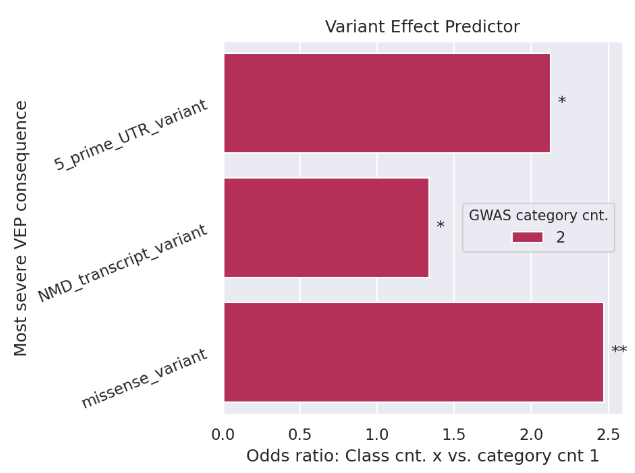
\includegraphics[width=\textwidth]{\floatRelativePath/pltbar_vep_consequence.py/vep.png}
%
\caption{Odds ratio of the variants annotated with given variant effect
predictor (VEP) consequence and given GWAS class count compared with non
pleiotropic variants with GWAS class count one. The significance is given for the
q-value with False discovery rate 5\%.}
\label{fig:vep_consequence}
%
\end{figure}

%%%%%%%%%%%%%%%%%%%%%%%%%%%%%%%%%%%%%%%%%%%%%%%%%%%%%%%%%%%%%%%%%%%%%%%%%%%%%%%%%
%%
%% Fig 6: Violin plots. eGenes, eTissues and gwas per variants
%%
%%%%%%%%%%%%%%%%%%%%%%%%%%%%%%%%%%%%%%%%%%%%%%%%%%%%%%%%%%%%%%%%%%%%%%%%%%%%%%%%%
%
\begin{figure}[!tbp]
\centering
%
\begin{subfigure}[]{.32\textwidth}
\textbf{a}
\\
\includegraphics[width=\textwidth]{\floatRelativePath/pltbar_x_per_variant_etissue_y_egene.py/plt.png}
\end{subfigure}
%
\begin{subfigure}[]{.32\textwidth}
\textbf{b}
\\
\includegraphics[width=\textwidth]{\floatRelativePath/pltbar_x_per_variant_egene_y_etissue.py/plt.png}
\end{subfigure}
%
%\begin{subfigure}[]{.32\textwidth}
%\textbf{c}
%\\
%\includegraphics[width=\textwidth]{\floatRelativePath/pltbar_x_per_variant_egene_etissue_y_gwas.py/plt.png}
%\end{subfigure}
%
\caption{Mean number of genes in eQTL-tissue pairs (\textbf{a}) and mean number of tissues in eQTL-gene pairs (\textbf{b}).} \label{fig:gwas_egene_etisue_per_variant}
%
\end{figure}

%%%%%%%%%%%%%%%%%%%%%%%%%%%%%%%%%%%%%%%%%%%%%%%%%%%%%%%%%%%%%%%%%%%%%%%%%%%%%%%%%
%%
%% Fig 7: TF count per GWAS class count
%%
%%%%%%%%%%%%%%%%%%%%%%%%%%%%%%%%%%%%%%%%%%%%%%%%%%%%%%%%%%%%%%%%%%%%%%%%%%%%%%%%%

\begin{figure}[!tbp]
\centering
%
\begin{subfigure}[]{.33\textwidth}
\textbf{a}
\\
\includegraphics[width=\textwidth]{\floatRelativePath/pltbox_x_per_rsid_y_remapnr.py/bxplt_remaptf_per_rsid_flank_10.png}
\end{subfigure}
%
\begin{subfigure}[]{.33\textwidth}
\textbf{b}
\\
\includegraphics[width=\textwidth]{\floatRelativePath/pltbar_x_per_variant_pleiotropy_y_remapcrm.py/remapcrm_flank10.png}
\end{subfigure}
%
\caption{Analysis of transcription factor binding.
\textbf{a}, Binding count of transcription factors in the region surrounding pleiotropic eQTLs with a radius of 50 bp as a function of the GWAS class count.
\textbf{b}, Odds ratio of eQTLs annotated as belonging to a cis regulatory modules vs. non-annotated.} \label{fig:freq_tf_per_variant}
%
\end{figure}

%%%%%%%%%%%%%%%%%%%%%%%%%%%%%%%%%%%%%%%%%%%%%%%%%%%%%%%%%%%%%%%%%%%%%%%%%%%%%%%%%
%%
%% Fig 8: beta and log pval
%%
%%%%%%%%%%%%%%%%%%%%%%%%%%%%%%%%%%%%%%%%%%%%%%%%%%%%%%%%%%%%%%%%%%%%%%%%%%%%%%%%%
%
%\begin{figure}[!tbp]
%\centering
%%
%\begin{subfigure}[]{.33\textwidth}
%\textbf{a}
%\\
%\includegraphics[width=\textwidth]{\floatRelativePath/pltbar_x_per_gwas_cat_y_beta.py/eqtl_beta.png}
%\end{subfigure}
%%
%\begin{subfigure}[]{.33\textwidth}
%\textbf{b}
%\\
%\includegraphics[width=\textwidth]{\floatRelativePath/pltbar_x_per_gwas_cat_y_beta.py/gwas_beta.png}
%\end{subfigure}
%
%\begin{subfigure}[]{.33\textwidth}
%\textbf{c}
%\\
%\includegraphics[width=\textwidth]{\floatRelativePath/pltbar_x_per_gwas_cat_y_logpval.py/eqtl.png}
%\end{subfigure}
%%
%\begin{subfigure}[]{.33\textwidth}
%\textbf{d}
%\\
%\includegraphics[width=\textwidth]{\floatRelativePath/pltbar_x_per_gwas_cat_y_logpval.py/gwas.png}
%\end{subfigure}
%
%\caption{eQTL and GWAS effect size/beta (\textbf{a,b}) and eQTL and GWAS significance/p-value (\textbf{c,d}) as a function of the GWAS class count.} \label{fig:beta_pval}
%%Correlation
%\end{figure}

%%%%%%%%%%%%%%%%%%%%%%%%%%%%%%%%%%%%%%%%%%%%%%%%%%%%%%%%%%%%%%%%%%%%%%%%%%%%%%%%%
%%
%% Fig 9: graphical conclusions
%%
%%%%%%%%%%%%%%%%%%%%%%%%%%%%%%%%%%%%%%%%%%%%%%%%%%%%%%%%%%%%%%%%%%%%%%%%%%%%%%%%%
%
\begin{figure}[!tbp]
\centering
%
\begin{subfigure}[]{\textwidth}

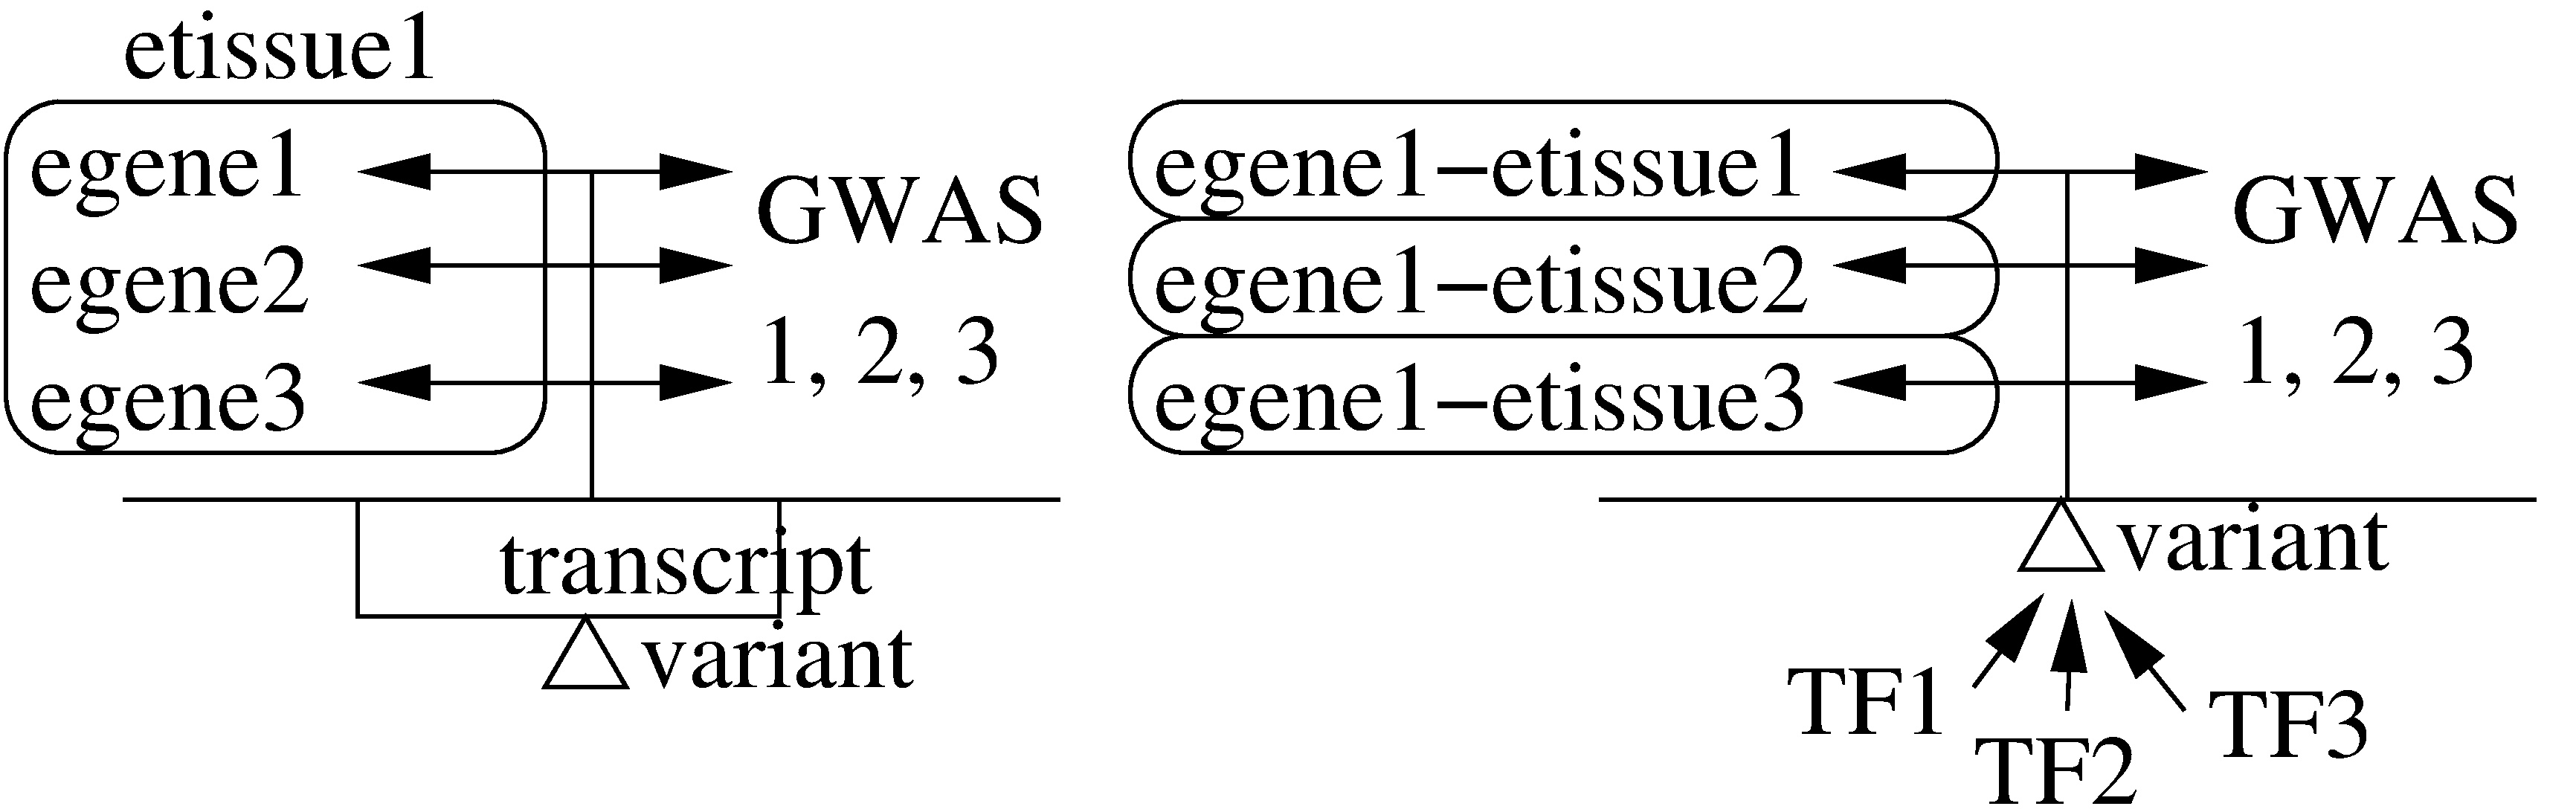
\includegraphics[width=\textwidth]{fig/graphical_summary.png}
\end{subfigure}

\caption{\textbf{Model of regulatory variant pleiotropy.} I have investigated three possible mechanisms of pleiotropy. \textbf{Left}, Pleiotropic variants have more eGenes that result in more functions and more phenotypes. This might arise from an enrichment of pleiotropic variants in splicing or 3' UTR regions. \textbf{Center}, I have also found that eGenes of pleiotropic variants are active in more etissues which result in more GWAS phenotypes. This might be explained from variants being bound by more transcription factors. \textbf{Left} Triplets of variant-eGene-eTissues are associated with more GWAS phenotypes, which directly affect the number of GWAS phenotypes. I have found that this might be explained by an enrichment of missense alleles.} \label{fig:beta}
%
\end{figure}




    \section*{Appendix}
    Text for this section\ldots

%%%%%%%%%%%%%%%%%%%%%%%%%%%%%%%%%%%%%%%%%%%%%%
%%                                          %%
%% Backmatter begins here                   %%
%%                                          %%
%%%%%%%%%%%%%%%%%%%%%%%%%%%%%%%%%%%%%%%%%%%%%%

    \begin{backmatter}

        \section*{Acknowledgements}%% if any
        Centre de Calcul Intensif d'Aix-Marseille is acknowledged for granting access to its high performance computing resources.
%
        I thank Sandrine Marquet, Marie Michel, Pascale Paul, Salvatore Spicuglia and Pascal Rihet for helpful discussions and Léopoldine Lecerf for a preliminary version of the colocalization pipeline developed during her internship.

%    \section*{Funding}%% if any
%    Text for this section\ldots

%    \section*{Abbreviations}%% if any
%    Text for this section\ldots

        \section*{Availability of data and materials}%% if any
        Text for this section\ldots

%    \section*{Ethics approval and consent to participate}%% if any
%    Text for this section\ldots

        \section*{Competing interests}
        The authors declare that they have no competing interests.

%    \section*{Consent for publication}%% if any
%    Text for this section\ldots

        \section*{Authors' contributions}
        Text for this section \ldots

%    \section*{Authors' information}%% if any
%    Text for this section\ldots

%%%%%%%%%%%%%%%%%%%%%%%%%%%%%%%%%%%%%%%%%%%%%%%%%%%%%%%%%%%%%
%%                  The Bibliography                       %%
%%                                                         %%
%%  Bmc_mathpys.bst  will be used to                       %%
%%  create a .BBL file for submission.                     %%
%%  After submission of the .TEX file,                     %%
%%  you will be prompted to submit your .BBL file.         %%
%%                                                         %%
%%                                                         %%
%%  Note that the displayed Bibliography will not          %%
%%  necessarily be rendered by Latex exactly as specified  %%
%%  in the online Instructions for Authors.                %%
%%                                                         %%
%%%%%%%%%%%%%%%%%%%%%%%%%%%%%%%%%%%%%%%%%%%%%%%%%%%%%%%%%%%%%

% if your bibliography is in bibtex format, use those commands:
        \bibliographystyle{bmc-mathphys} % Style BST file (bmc-mathphys, vancouver, spbasic).
        \bibliography{ms_pleiotropy}      % Bibliography file (usually '*.bib' )
% for author-year bibliography (bmc-mathphys or spbasic)
% a) write to bib file (bmc-mathphys only)
% @settings{label, options="nameyear"}
% b) uncomment next line
%\nocite{label}

% or include bibliography directly:
% \begin{thebibliography}
% \bibitem{b1}
% \end{thebibliography}

%%%%%%%%%%%%%%%%%%%%%%%%%%%%%%%%%%%
%%                               %%
%% Figures                       %%
%%                               %%
%% NB: this is for captions and  %%
%% Titles. All graphics must be  %%
%% submitted separately and NOT  %%
%% included in the Tex document  %%
%%                               %%
%%%%%%%%%%%%%%%%%%%%%%%%%%%%%%%%%%%

%%
%% Do not use \listoffigures as most will included as separate files

        \section*{Figures}

        \begin{figure}[h!]
            \caption{Histogram showing the percentage of GWAS with the percentage of their tophits colocalized with eQTLs.
            I have excluded tophits in in the MHC locus in chromosome 6 between 25,000,000 and 35,000,000,
                because this locus is not included in the colocalization pipeline.}
            \label{fig:hist_perc_tophits_eqtl_excl_mhc}
        \end{figure}

%%%%%%%%%%%%%%%%%%%%%%%%%%%%%%%%%%%
%%                               %%
%% Tables                        %%
%%                               %%
%%%%%%%%%%%%%%%%%%%%%%%%%%%%%%%%%%%

%% Use of \listoftables is discouraged.
%%
        \section*{Tables}

        %%%%%%%%%%%%%%%%%%%%%%%%%%%%%%%%%%%%%%%%%%%%%%%%%%%%%%%%%%%%%%%%%%%%%%%%%%%%%%%%
%
% Tab 1: Representative pleiotropic eQTLs of cytobands
%
%%%%%%%%%%%%%%%%%%%%%%%%%%%%%%%%%%%%%%%%%%%%%%%%%%%%%%%%%%%%%%%%%%%%%%%%%%%%%%%%

\begin{table}[!ht]
    \centering
    \scriptsize

    \csvreader[separator=tab,
    tabular=crclcp{0.4\textwidth},
    late after last line=\\\hline,
    head,
    table head=\\\hline \bfseries Chrom. & \bfseries Pos (hg38) & \bfseries Cytoband & \bfseries RSID & \bfseries Gene marker& \bfseries Trait categories\\\hline,
    ]{\floatRelativePath/cmpt_count_per_rsid.py/count_per_rsid_gwas_ms.tsv}{}% use head of csv as column names
        {\csvcoli\ & \csvcolii\ & \csvcoliii\ & \csvcoliv\ & \csvcolv\ & \csvcolvi}% specify your coloumns here
    %
    \vspace{15pt}
    %
    \caption{
%        Represantive pleiotropic eQTLs involved in four GWAS categories in different cytobands.
%    The gene marker is the eQTL gene with the highest PubMed publication count.
%    The whole list is given in the Supplementary table ST2.
    }
    \label{tab:pleitropic_eqtls}
\end{table}

%%%%%%%%%%%%%%%%%%%%%%%%%%%%%%%%%%%%%%%%%%%%%%%%%%%%%%%%%%%%%%%%%%%%%%%%%%%%%%%%
%
% Tab 2: Region containing most pleiotropic eQTLs
%
%%%%%%%%%%%%%%%%%%%%%%%%%%%%%%%%%%%%%%%%%%%%%%%%%%%%%%%%%%%%%%%%%%%%%%%%%%%%%%%%

\begin{table}[!ht]
    \centering
    \scriptsize
    \csvreader[
        separator=tab,
        tabular=p{0.03\textwidth}p{0.1\textwidth}p{0.1\textwidth}p{0.06\textwidth}p{0.08\textwidth}p{0.45\textwidth}p{0.08\textwidth}p{0.08\textwidth},
        late after last line=\\\hline,
        head,
        table head=\\\hline \bfseries Chr. & \bfseries Start & \bfseries End & \bfseries Cytob. & \bfseries Marker eQTL gene & \bfseries Trait categories & \bfseries Length & \bfseries eQTLs cnt.\\\hline,
    ]{\floatRelativePath/cmpt_pleiotropic_regions.py/100000/region_window_ms.tsv}{}% use head of csv as column names
    {\csvcoli\ & \csvcolii\ & \csvcoliii\ & \csvcoliv\ & \csvcolv\ & \csvcolvi\ & \csvcolvii\ & \csvcolviii}% specify your coloumns here
    %
    \vspace{15pt}
    %
    \caption{
%        Pleiotropic regions involving 6 or more GWAS classes. These regions were built with a sliding window of 1e5 nt. Genomic coordinates are given for the hg38 assembly.
    }\label{tab:pleiotropic_regions}
    %
\end{table}


%%%%%%%%%%%%%%%%%%%%%%%%%%%%%%%%%%%
%%                               %%
%% Additional Files              %%
%%                               %%
%%%%%%%%%%%%%%%%%%%%%%%%%%%%%%%%%%%

        \section*{Additional Files}
        \subsection*{Additional file 1: Table S1.}
        Classification of eQTL tissues and cell types. The first six were downloaded from the EBI eQTL repository.
        The 7th column "etissue\_category\_term" is used here to compute tissue diversity.

        \subsection*{Additional file 2: Table S2.}
        Metadata and classification of GWAS.

        \subsection*{Additional file 3: Table S3.}
        Percentage of tophits per GWAS that colocalized with at least one eQTL.

        \subsection*{Additional file 4: Table S4.}
        Count and list of GWAS phenotypes, egenes and etissues for each eQTL/GWAS variant.

        \subsection*{Additional file 5: Table S5.}
        Count and list of GWAS phenotypes, egene symbols and ENSEMBL IDs and etissue classes for each pleiotropic region.

    \end{backmatter}
\end{document}
